\documentclass[PianoDiQualifica.tex]{subfiles}
\begin{document}
	\begin{appendices}
		
		\chapter{Ciclo di Deming o PDCA}
		Ogni processo deve essere organizzato basandosi sul principio del miglioramento continuo (o \citGloss{ciclo di Deming}):
		\begin{description}
			\item [Plan (pianificare)]: viene definito un piano che basandosi sulla definizione di problemi e obiettivi pianifica compiti, assegna responsabilità, studia il caso, analizza le cause della criticità e definisce azioni correttive; 
			\item [Do (eseguire)]: vengono implementate le attività secondo le linee definite durante la fase Plan;
			\item [Check (valutare)]: viene verificato l'esito delle azioni di miglioramento rispetto alle attese;
			\item [Act (agire)]: vengono applicate le correzioni necessarie per colmare le carenze rilevate e vengono standardizzate le attività correttamente eseguite.
		\end{description}
		
		\begin{figure}[htbp]
			\begin{center}
				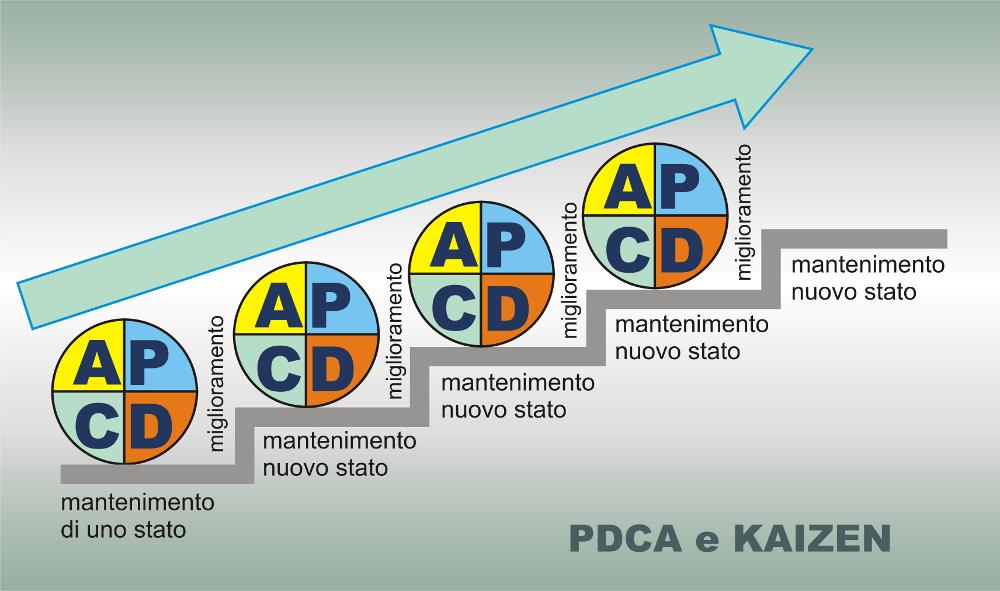
\includegraphics[width=0.7\linewidth]{PDCAkaizen}
				\caption[Ciclo di Deming]{Ciclo di Deming}
				\label{fig:pdca}
			\end{center}
		\end{figure}
		
		\chapter{ISO/IEC 15504}
		Lo standard ISO/IEC 15504 contiene un modello di riferimento che definisce 
		\begin{itemize}
			\item Process dimension;
			\item Capability dimension.
		\end{itemize}
		
		La dimensione di processo divide i processi in cinque categorie:
		\begin{itemize}
			\item Customer-supplier;
			\item Engineering;
			\item Supporting;
			\item Management;
			\item Organization.
		\end{itemize}
		
		Per ogni processo, lo standard ISO/IEC 15504 definisce dei livelli di capacità:
		\begin{description}
			\item [\normalfont Livello 5] \textbf{Optimizing process}: il processo è continuamente migliorato;
			\item [\normalfont Livello 4] \textbf{Predictable process}: il processo è adottato sistematicamente, entro limiti definiti;
			\item [\normalfont Livello 3] \textbf{Established process}: un processo stabilito si basa su un processo standard;
			\item [\normalfont Livello 2] \textbf{Managed process}: il processo è gestito e i prodotti sono stabiliti, controllati e mantenuti;
			\item [\normalfont Livello 1] \textbf{Performed process}: il processo è implementato e raggiunge lo scopo stabilito;
			\item [\normalfont Livello 0] \textbf{Incomplete process}: il processo non è implementato o non raggiunge lo scopo stabilito.\\
		\end{description}
		
		La capacità dei processi viene misurata attraverso degli attributi di processo.
		\begin{itemize}
			\item Livello 1
			\begin{itemize}
				\item \textbf{Process performance:} capacità di un processo di raggiungere gli obiettivi trasformando input identificabili in output identificabili;
			\end{itemize}
			\item Livello 2
			\begin{itemize}
				\item \textbf{Performance management:} capacità del processo di elaborare un prodotto coerente con gli obiettivi fissati;
				\item \textbf{Work product management:} capacità del processo di elaborare un prodotto documentato, controllato e verificato;
			\end{itemize}
			\item Livello 3
			\begin{itemize}
				\item \textbf{Process definition:} l'esecuzione del processo si basa su standard di processo per raggiungere i propri obiettivi;
				\item \textbf{Process deployment:} capacità del processo di attingere a risorse tecniche e umane appropriate per essere attuato efficacemente;
			\end{itemize}
			\item Livello 4
			\begin{itemize}
				\item \textbf{Process measurement:} gli obiettivi e le misure di prodotto e di processo vengono usati per garantire il raggiungimento dei traguardi definiti in supporto ai target aziendali;
				\item \textbf{Process control:} il processo viene controllato tramite misure di prodotto e processo per effettuare correzioni migliorative al processo stesso;
			\end{itemize}
			\item Livello 5
			\begin{itemize}
				\item \textbf{Process innovation:} i cambiamenti strutturali, di gestione e di esecuzione vengono gestiti in modo controllato per raggiungere i risultati fissati;
				\item \textbf{Process optimization:} le modifiche al processo sono identificate e implementate per garantire il miglioramento continuo nella realizzazione degli obiettivi di business dell'organizzazione. 
			\end{itemize}
		\end{itemize}
		
		Ogni attributo consiste di una o più pratiche generiche che sono ulteriormente elaborate in indicatori pratici per aiutare la valutazione delle performance, sotto forma di indici N-P-L-F:
		\begin{itemize}
			\item Non soddisfatto (0 - 15\%);
			\item Parzialmente soddisfatto ($ > $15\% - 50\%);
			\item Largamente soddisfatto ($ > $50\% - 85\%);
			\item Totalmente soddisfatto ($ > $85\% - 100\%)
		\end{itemize}
		
	\end{appendices}
\end{document}